\documentclass[10pt]{beamer}

\usetheme{metropolis}
\usepackage{appendixnumberbeamer}

\usepackage{booktabs}
\usepackage[scale=2]{ccicons}

\usepackage{pgfplots}
\usepgfplotslibrary{dateplot}

\usepackage{xspace}

\usepackage{tikz}
    \usetikzlibrary{positioning}

%\usepackage{listings}
\usepackage{minted}

\usepackage{bm}%................................. Bold math symbols (after fonts)

\setbeamercolor{normal text}{bg=white}





\title{EML4930/EML6934: Lecture 04}
\subtitle{Introduction to NumPy and matrix operations}
\date{September 21, 2017}
%\author{CJ}
\author{Charles Jekel}
%\titlegraphic{\includegraphics{images/avatarCropped.png}\vspace{58cm}}
%\institute{1. University of Florida\\ 2. Stellenbosch University, South Africa}

% \titlegraphic{\hfill\includegraphics[height=1.5cm]{logo.pdf}}

\begin{document}

\maketitle

\begin{frame}{Quiz at the end of next class}
There will be a quiz at the end of next class. 

The quiz will be closed notes!

The quiz will be 3 short questions. 

10 sample quiz questions are posted online. You should know how to answer each one of these questions. The 3 questions asked will be very similar to these 10 questions.
\end{frame}

\begin{frame}[fragile]{Concerns about HW?}
The Fibonacci problem can be coded without the need of iterating through an index. If you are working with lists in Python you may not need the list index!

\begin{minted}
{python}
F = [0, 1, 1]
#    Calculate the next 20 items in the Fibonacci sequence
for i in range(20):
    F.append(F[-1]+F[-2])
\end{minted}
\end{frame}

\begin{frame}{Reference for this lecture}
This lecture will cover chapter 2 of Python Data Science Handbook by VanderPlas. 

\url{http://nbviewer.jupyter.org/github/jakevdp/PythonDataScienceHandbook/blob/master/notebooks/Index.ipynb}
\end{frame}

\begin{frame}{NumPy - \url{http://numpy.org}}
NumPy is the fundamental package for scientific computing with Python. It contains among other things:
\begin{itemize}
\item a powerful N-dimensional array object
\item sophisticated (broadcasting) functions
\item tools for integrating C/C++ and Fortran code
\item useful linear algebra, Fourier transform, and random number capabilities
\item documentation \url{https://docs.scipy.org/doc/numpy-1.13.0/reference/index.html}
\end{itemize}
\end{frame}

\begin{frame}{If you're coming from MATLAB read}
\url{https://docs.scipy.org/doc/numpy-dev/user/numpy-for-matlab-users.html}
\end{frame}

\begin{frame}[fragile]{Importing NumPy}
\begin{minted}
{python}
import numpy as np
\end{minted}

This is the most standard form of how to import the numpy library.
\end{frame}


\begin{frame}[fragile]{What is a NumPy array?}
	\begin{alertblock}{NumPy ndarray()}
A n-dimensional arrays of homogeneous data types. 
	\end{alertblock}

\begin{itemize}
\item The \textit{ndarray} object is the core of NumPy.
\item \textit{ndarray} has become the standard Python vector/matrix/tensor types.
\item Elements of \textit{ndarray} must have the same data type.
\item Mathematical operations on \textit{ndarray} are more efficient than built-in Python functions.
\item Much of the code was created in compiled code for performance. 
\item Documentation \url{https://docs.scipy.org/doc/numpy-1.10.0/reference/arrays.ndarray.html}
\end{itemize}
\end{frame}

\begin{frame}[fragile]{NumPy array attributes - memory layout}
The following attributes contain information about the memory layout of the array:
\begin{itemize}
\item ndarray.flags - Information about the memory layout of the array.
\item ndarray.shape -	Tuple of array dimensions.
\item ndarray.strides -	Tuple of bytes to step in each dimension when traversing an array.
\item ndarray.ndim -	Number of array dimensions.
\item ndarray.data -	Python buffer object pointing to the start of the array’s data.
\item ndarray.size -	Number of elements in the array.
\item ndarray.itemsize - 	Length of one array element in bytes.
\item ndarray.nbytes - 	Total bytes consumed by the elements of the array.
\item ndarray.base -	Base object if memory is from some other object.
\end{itemize}
\end{frame}

\begin{frame}[fragile]{NumPy array attributes - other attributes}
The following attributes contain information about the memory layout of the array:
\begin{itemize}
\item ndarray.dtype -	Data-type of the array’s elements.
\item ndarray.T -	Same as self.transpose(), except that self is returned if self.ndim $<$ 2.
\item ndarray.real - 	The real part of the array.
\item ndarray.imag -	The imaginary part of the array.
\item ndarray.flat -	A 1-D iterator over the array.
\item ndarray.ctypes -	An object to simplify the interaction of the array with the ctypes module.
\end{itemize}
\end{frame}

\begin{frame}{NumPy array methods - array conversion 1 of 2}
\begin{itemize}
\item ndarray.item(*args) - 	Copy an element of an array to a standard Python scalar and return it.
\item ndarray.tolist() -	Return the array as a (possibly nested) list.
\item ndarray.itemset(*args) -	Insert scalar into an array (scalar is cast to array's dtype, if possible) There must be at least 1 argument, and define the last argument as item.
\item ndarray.tostring([order]) -	Construct Python bytes containing the raw data bytes in the array.
\item ndarray.tobytes([order]) - 	Construct Python bytes containing the raw data bytes in the array.
\item ndarray.tofile(fid[, sep, format]) -	Write array to a file as text or binary (default).
\item ndarray.dump(file) -	Dump a pickle of the array to the specified file.
\item ndarray.dumps() -	Returns the pickle of the array as a string.
\item ndarray.astype(dtype[, order, casting, ...]) -	Copy of the array, cast to a specified type.
\end{itemize}
\end{frame}

\begin{frame}{NumPy array methods - array conversion 2 of 2}
\begin{itemize}
\item ndarray.byteswap(inplace) -	Swap the bytes of the array elements Toggle between low-endian and big-endian data representation by returning a byteswapped array, optionally swapped in-place.
\item ndarray.copy([order]) -	Return a copy of the array.
\item ndarray.view([dtype, type]) -	New view of array with the same data.
\item ndarray.getfield(dtype[, offset]) -	Returns a field of the given array as a certain type.
\item ndarray.setflags([write, align, uic]) -	Set array flags WRITEABLE, ALIGNED, and UPDATEIFCOPY, respectively.
\item ndarray.fill(value) -	Fill the array with a scalar value.
\end{itemize}
\end{frame}

\begin{frame}{NumPy array methods - shape manipulation}
\begin{itemize}
\item ndarray.reshape(shape[, order]) -	Returns an array containing the same data with a new shape.
\item ndarray.resize(new\_shape[, refcheck]) - 	Change shape and size of array in-place.
\item ndarray.transpose(*axes) -	Returns a view of the array with axes transposed.
\item ndarray.swapaxes(axis1, axis2) -	Return a view of the array with axis1 and axis2 interchanged.
\item ndarray.flatten([order]) -	Return a copy of the array collapsed into one dimension.
\item ndarray.ravel([order]) -	Return a flattened array.
\item ndarray.squeeze([axis]) -	Remove single-dimensional entries from the shape of a.
\end{itemize}
\end{frame}

\begin{frame}{Numpy array methods - methods that are also functions}
\begin{columns}
\begin{column}{0.3\textwidth}
\begin{itemize}
\item all
\item any
\item argmax
\item argmin
\item argpartition
\item argsort
\item choose
\item clip
\item compress
\item copy
\item cumprod
\item cumsum
\item diagonal
\end{itemize}

\end{column}
\begin{column}{0.3\textwidth} 
\begin{itemize}
\item imag
\item max
\item mean
\item min
\item nonzero
\item partition
\item prod
\item ptp 
\item put
\item ravel
\item real
\item repeat
\end{itemize}
\end{column}
\begin{column}{0.3\textwidth} 
\begin{itemize}
\item reshape
\item round
\item searchsorted
\item sort
\item squeeze
\item std
\item sum
\item swapaxes
\item take
\item trace
\item transpose
\item var
\end{itemize}
\end{column}
\end{columns}
\end{frame}

\begin{frame}{NumPy array data types - 1 of 2}
\begin{table}
\begin{tabular}{ll}
\textbf{Type} & \textbf{Description}  \\
\hline
bool\_ 	  &  Boolean (True or False) stored as a byte \\
int\_ 	    &  Default integer type (normally either int64 or int32) \\
intc 	    &  Identical to C int (normally int32 or int64) \\
intp 	    &  Integer used for indexing (normally either int32 or int64) \\
int8 	    &  Byte (-128 to 127) \\
int16 	  &  Integer (-32768 to 32767) \\
int32 	  &  Integer (-2147483648 to 2147483647) \\
int64 	  &  Integer (-9223372036854775808 to 9223372036854775807) \\
uint8 	  &  Unsigned integer (0 to 255) \\
uint16 	  &  Unsigned integer (0 to 65535) \\
uint32 	  &  Unsigned integer (0 to 4294967295) \\
uint64 	  &  Unsigned integer (0 to 18446744073709551615) \\
\end{tabular}
\end{table}
\end{frame}
\begin{frame}{NumPy array data types - 2 of 2}
NumPy arrays support a larger variety of data types than the default Python!
\begin{table}
\begin{tabular}{ll}
\textbf{Type} & \textbf{Description}  \\
\hline
float\_ 	  &  Shorthand for float64. \\
float16 	&  Half precision: sign bit, 5 bits exponent, 10 bits mantissa \\
float32 	&  Single precision: sign bit, 8 bits exponent, 23 bits mantissa \\
float64 	&  Double precision: sign bit, 11 bits exponent, 52 bits mantissa \\
complex\_ 	&  Shorthand for complex128. \\
complex64 &	Complex number, represented by two 32-bit floats  \\
complex128 & 	Complex number, represented by two 64-bit floats  \\
\end{tabular}
\end{table}
\end{frame}

\begin{frame}[fragile]{NumPy array creation - from lists}
Use \mint{python}|np.array(list)|
to create an array from a Python list

Examples:
\begin{minted}
{python}
# one dimensional array shape (4,)
x = np.array([1, 2, 4, 6])

# two dimensional array shape (2,2)
y = np.array([[1 ,2], [2, 3]])

# three dimensional array - shape (2,2,2)
z = np.array([[[1 ,2], [2, 3]], [[1 ,2], [2, 3]]])
\end{minted}
\end{frame}

\begin{frame}[fragile]{NumPy array creation - specify data type}
You can specify the data type of the array using \mint{python}|np.array(list, dtype=)|

Examples:
\begin{minted}
{python}
# one dimensional array - Byte
x = np.array([1, 2, 4, 6], dtype='int8')

# two dimensional array - Single precision
y = np.array([1, 2, 4, 6], dtype='float32')

# three dimensional array - Double precision
z = np.array([1, 2, 4, 6], dtype='float64')
\end{minted}

\end{frame}

\begin{frame}[fragile]{NumPy array creation - display data type}
You can view the data type with \mint{python}|ndarray.dtype)|

Examples:
\begin{minted}
{python}
in : x.dtype
out: dtype('int8')

in : y.dtype
out: dtype('float32')

in : z.dytpe
out: dtype('float64')
\end{minted}
\end{frame}

\begin{frame}[fragile]{Default data types follow python convention}

If you include a decimal point NumPy array will default to double precision floating point.

Examples:
\begin{minted}
{python}
in : a = np.array(1); a.dtype
out: dtype('int32')

in : b = np.array(1.); b.dtype
out: dtype('float64')

in : c = np.array([1,1.]); c.dtype
out: dtype('float64')

in : d = np.array([1., 1, 1, 1, 1, 1, 1]); d.dtype
out: dtype('float64')
\end{minted}
\end{frame}

\begin{frame}[fragile]{NumPy array creation - from scratch 1 of 3}
These default to double precision floating point unless otherwise specified.
\begin{minted}
{python}
# Create a length-10 integer array filled with zeros
np.zeros(10, dtype=int)

# Create a 3x5 floating-point array filled with 1s
np.ones((3, 5), dtype=float)

# Create a 3x5 array filled with 3.14
np.full((3, 5), 3.14)

# Create an array filled with a linear sequence
# Starting at 0, ending at 20, stepping by 2        
np.arange(0, 20, 2)
\end{minted}
\end{frame}

\begin{frame}[fragile]{NumPy array creation - from scratch 2 of 3}
\begin{minted}
{python}
# Create an array of five values evenly spaced between 0 and 1
np.linspace(0, 1, 5)

# Create a 3x3 array of uniformly distributed
# random values between 0 and 1
np.random.random((3, 3))

# Create a 3x3 array of normally distributed random values
# with mean 0 and standard deviation 1
np.random.normal(0, 1, (3, 3))

# Create a 3x3 array of random integers in the interval [0, 10)
np.random.randint(0, 10, (3, 3))

# Create a 3x3 identity matrix
np.eye(3)
\end{minted}
\end{frame}

\begin{frame}[fragile]{NumPy array creation - from scratch 3 of 3}
\begin{minted}
{python}
# Create an uninitialized array of three integers
# The values will be whatever happens to already exist at that
# memory location        
np.empty(3)
\end{minted}
\end{frame}

\begin{frame}[fragile]{Seeding NumPy pseudorandom number generator}
Use seed to ensure that the arrays are the same for each time the code is run.

\begin{minted}
{python}
# seed for reproducibility
np.random.seed(0)  

# One-dimensional array 
x1 = np.random.randint(10, size=6)

# Two-dimensional array        
x2 = np.random.randint(10, size=(3, 4))

# Three-dimensional array          
x3 = np.random.randint(10, size=(3, 4, 5))  
\end{minted}
\end{frame}

\begin{frame}[fragile]{NumPy array - useful attributes}
\begin{minted}
{python}
# the number of dimensions
print("x3 ndim: ", x3.ndim)

# the size of each dimension of the array 
print("x3 shape:", x3.shape)

# the total size of the array   
print("x3 size: ", x3.size)

# the item size (in bytes) of each array element       
print("itemsize:", x3.itemsize, "bytes")

# the total size (in bytes) of the array   
print("itemsize:", x3.nbytes, "bytes")
\end{minted}
\end{frame}

\begin{frame}[fragile]{NumPy array indexing - one dimensional}
One dimensional arrays index just like lists
\begin{minted}
{python}
x = np.array([2, 3, 4, 9])

# print the first item
print(x[0])

# print the second item
print(x[1])

# print the last item
print(x[-1])
\end{minted}
\end{frame}

\begin{frame}[fragile]{NumPy array indexing - two dimensional}
Two dimensional arrays also index just like lists! 
\begin{minted}
{python}
y = np.array([[1,2], [3,4]])

# print 1 from y
print(y[0,0])

# print 2 from y
print(y[0,1])

# print 3 from y
print(y[1,0])

# print 4 from y
print(y[1,1])
\end{minted}
\end{frame}

\begin{frame}[fragile]{NumPy array slicing - just like list slicing!}
\begin{minted}
{python}
in : x = np.array([0, 1, 2, 3, 4, 5, 6, 7, 8, 9])
in : x[:5]  # first five elements
out: array([0, 1, 2, 3, 4])

in : x[5:]  # elements after index 5
out: array([5, 6, 7, 8, 9])

in : x[4:7]  # middle subarray
out: array([4, 5, 6])

in : x[::2]  # every other element
out: array([0, 2, 4, 6, 8])

in : x[1::2]  # every other element, starting at index 1
out: array([1, 3, 5, 7, 9]) 

in : x[::-1]  # all elements, reversed
out: array([9, 8, 7, 6, 5, 4, 3, 2, 1, 0])
\end{minted}
\end{frame}

\begin{frame}[fragile]{NumPy array - rows and columns of}
\begin{minted}
{python}
in : x = np.array([[12,  5,  2,  4],
                   [ 7,  6,  8,  8],
                   [ 1,  6,  7,  7]])

# first column of x
x[:,0]

# second column of x
x[:,1]

# third row of x
x[2,:]

# first row of x
x[0,:]
\end{minted}
\end{frame}

\begin{frame}[fragile]{NumPy array - assigning individual values}
\begin{minted}
{python}
in : x = np.array([[12,  5,  2,  4],
                   [ 7,  6,  8,  8],
                   [ 1,  6,  7,  7]])

x[0,0] = 0
x[0,1] = 1
x[0,2] = 2
x[0,3] = 3
print(x)

out: array([[ 0,  1,  2,  3],
            [ 7,  6,  8,  8],
            [ 1,  6,  7,  7]])
\end{minted}
\end{frame}

\begin{frame}[fragile]{NumPy arrays pass by reference!}
use copy() if you want a copy of the data!

\begin{minted}
{python}
a = np.ones(3)
b = a
c = a.copy()

a *= 7
print('a:', a)
print('b:', b)
print('c:', c)
\end{minted}
\end{frame}

\begin{frame}{NumPy aggregration functions}
\begin{table}
\begin{tabular}{lll}
\textbf{Function} & \textbf{NaN-safe} & \textbf{Description}  \\
\hline
np.sum          & np.nansum        & Compute sum of elements\\
np.prod         & np.nanprod       & Compute product of elements\\
np.mean         & np.nanmean       & Compute median of elements \\
np.std          & np.nanstd        & Compute standard deviation \\
np.var          & np.nanvar        & Compute variance \\
np.min          & np.nanmin        & Find minimum value \\
np.max          & np.nanmax        & Find maximum value \\
np.argmin       & np.nanargmin     & Find index of minimum value \\
np.argmax       & np.nanargmax     & Find index of maximum value \\
np.median       & np.nanmedian     & Compute median of elements \\
np.percentile   & np.nanpercentile & Compute rank-based statistics of elements \\
np.any          & N/A Evaluate     & whether any elements are true \\
np.all          & N/A Evaluate     & whether all elements are true\\
\end{tabular}
\end{table}
\end{frame}

\begin{frame}[fragile]{NumPy useful functions}
\begin{minted}
{python}
np.abs(x) # absolute value

# trig functions
np.sin(x)
np.cos(x)
np.tan(x)
np.arcsin(x)
np.arccos(x)
np.arctan(x)


np.exp(x)  # e^x
np.log(x)  # natural log
np.log2(x) # log base 2
np.log10(x)# log base 10
\end{minted}
\end{frame}

\begin{frame}[fragile]{NumPy arrays - arithmetic operators}
\begin{table}
\begin{tabular}{ll}
\textbf{Operator} & \textbf{Description}  \\
\hline
 + & Addition (e.g., 1 + 1 = 2)\\
 - & Subtraction (e.g., 3 - 2 = 1) \\
 - & Unary negation (e.g., -2) \\
 * & Multiplication (e.g., 2 * 3 = 6) \\
/  & Division (e.g., 3 / 2 = 1.5) \\
// & Floor division (e.g., 3 // 2 = 1) \\
** & Exponentiation (e.g., 2 \*\* 3 = 8) \\
 \% & Modulus/remainder (e.g., 9 \% 4 = 1)\\
\end{tabular}
\end{table}
\end{frame}

\begin{frame}[fragile]{NumPy arrays - element wise math}
\begin{minted}
{python}
in :
a = np.array([2, 4, 6, 8])
b = np.array([3, 4, 5, 6])

print(a+b)
print(a-b)
print(a*b)
print(a**b)

out: 
[ 5  8 11 14]
[-1  0  1  2]
[ 6 16 30 48]
[     8    256   7776 262144]
\end{minted}
\end{frame}

\begin{frame}[fragile]{NumPy arrays - element wise math}
\begin{minted}
{python}
in :
a = np.array([[2, 4],[6, 8]])
b = np.array([[3, 4],[5, 6]])
print(a+b)
print(a-b)
print(a*b)
print(a**b)

out: 
[[ 5  8]
 [11 14]]
[[-1  0]
 [ 1  2]]
[[ 6 16]
 [30 48]]
[[     8    256]
 [  7776 262144]]
\end{minted}
\end{frame}

\begin{frame}[fragile]{NumPy arrays - dot product}
Use np.dot(a,b) to take the dot product of arrays a and b

\begin{minted}
{python}
in :
a = np.array([2, 4, 6, 8])
b = np.array([3, 4, 5, 6])
print(np.dot(a,b))

out: 100
\end{minted}
\end{frame}

\begin{frame}[fragile]{NumPy arrays - dot product for matrix multiplication}
The dot product of two dimensional arrays is matrix multiplication

\begin{minted}
{python}
in :
x = np.array([[4, 5, 2],
              [7, 7, 1],
              [9, 1, 7]])
y = np.eye(3)

print(np.dot(x,y))

out: 
[[4, 5, 2],
 [7, 7, 1],
 [9, 1, 7]])
\end{minted}
\end{frame}

\begin{frame}[fragile]{NumPy linear algebra - decomposition}
\begin{table}
\begin{tabular}{ll}
\textbf{function} & \textbf{Description}  \\
\hline
np.linalg.cholesky(a) & Cholesky decomposition \\
np.linalg.qr(a[,mode]) & qr factorization \\
np.linalg.svd(a[, full\_matrices, compute\_uv]) & Singular value decomposition \\
\end{tabular}
\end{table}
\end{frame}

\begin{frame}[fragile]{NumPy linear algebra - eigenvalues}
\begin{minted}
{python}
in :
w, v = np.linalg.eig(np.diag((1, 2, 3)))

print(w)
print(v)

out: 
array([ 1.,  2.,  3.])
array([[ 1.,  0.,  0.],
       [ 0.,  1.,  0.],
       [ 0.,  0.,  1.]])
\end{minted}
\end{frame}

\begin{frame}{NumPy linear algebra - norms and other numbers}
\begin{table}
\begin{tabular}{ll}
\textbf{Function} & \textbf{Description}  \\
\hline
np.linalg.norm(x) 	     & Matrix or vector norm.\\
np.linalg.cond(x) 	     & Compute the condition number of a matrix.\\
np.linalg.det(a) 	       & Compute the determinant of an array.\\
np.linalg.matrix\_rank(M) & Return matrix rank of array using SVD method.\\
np.linalg.slogdet(a) 	   & Sign and $\ln$ of the determinant of an array.\\
np.trace(a) 	           & Return the sum along diagonals of the array.\\
\end{tabular}
\end{table}
\end{frame}

\begin{frame}{NumPy linear algebra - solving equations and inverting matrices}
\begin{table}
\begin{tabular}{ll}
\textbf{Function} & \textbf{Description}  \\
\hline
np.linalg.solve(a, b) 	            &  Solve a linear matrix equation\\
np.linalg.tensorsolve(a, b[, axes]) &	Solve the tensor equation a x = b for x\\
np.linalg.lstsq(a, b[, rcond]) 	    &  least-squares solution to a linear equation\\
np.linalg.inv(a) 	                  & multiplicative) inverse of a matrix\\
np.linalg.pinv(a[, rcond])    	    &  (Moore-Penrose) pseudo-inverse of a matrix\\
np.linalg.tensorinv(a[, ind]) 	    &  ‘inverse’ of an N-dimensional array\\
\end{tabular}
\end{table}
\end{frame}

\begin{frame}[fragile]{Don't invert arrays! Use solve!}
np.linalg.solve automatically uses parallel processing if it suspects using multiple threads will be faster!
\begin{minted}
{python}
F = np.array([[2.0, 3.0],
              [-2.0,9.0]])
c = np.array([ 12.9,  12.3])

# solve the equation Fa = c for a
a = np.linalg.solve(F,c)

# check the solution
print(np.dot(F,a))
\end{minted}
\end{frame}



%\begin{frame}[fragile]{Objects - everything in Python is an object}
%In this example x isn't really a string. It is an object containing a collection of functions
%\begin{minted}
%{python}
%in : x = 'hello world'
%
%in : dir(x)
%
%\end{minted}
%
%dir(object) returns an alphabetized list of the attributes of the object
%\end{frame}
%
%\begin{frame}{Object Oriented Programming - OOP}
%	\begin{alertblock}{Object Oriented Programming}
%A programming paradigm in which code related to a particular \textit{object} is grouped together. 
%	\end{alertblock}
%\begin{itemize}
%\item Class - the \textbf{definition} of an Object
%\item Object - an \textbf{instance} of a Class
%\item Everything in Python is an object
%\item Advantage - less duplicate code
%\item Disadvantage - performance issues with OOP
%\end{itemize}
%\end{frame}
%
%\begin{frame}{Objects and dogs...}
%Imagine you had to write a veterinarian program about dogs. What functions and attributes would all dogs have in common? 
%\begin{figure}
%	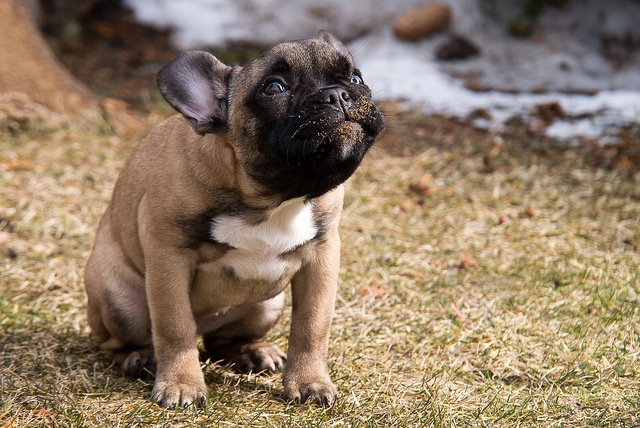
\includegraphics[width=1.0\textwidth]{figs/dog.jpg}
%\end{figure}
%\end{frame}
%
%\begin{frame}[fragile]{Use class to create a new form of object}
%Some reading: \url{https://docs.python.org/3/tutorial/classes.html} \url{http://anandology.com/python-practice-book/object_oriented_programming.html}
%
%I like this idea of creating a bank account to explain how to use class.
%\end{frame}
%
%\begin{frame}[fragile]{Creating a bank account object}
%\begin{minted}
%{python}
%class bank_account:
%    def __init__(self, initial_balance=0.0):
%        self.balance = initial_balance
%john = bank_account()
%\end{minted}
%
%\begin{itemize}
%\item use class to create an object named bank\_account
%\item def \_\_init\_\_() is an initialization function that is run automatically on a new instance
%\item you can add required and optional variables to the \_\_init\_\_() function
%\item self is the naming convention in python of objects own instance (it's self)
%\item self is the first variable in your functions of your object
%\item pass self to your object's functions if you need access to your object's attributes\
%\item balance is an attribute of the object
%\item a new instance of the object is created by calling bank\_account()
%\end{itemize}
%\end{frame}
%
%\begin{frame}[fragile]{adding a withdrawn and deposit function}
%\begin{minted}
%{python}
%class bank_account:
%    def __init__(self, initial_balance=0.0):
%        self.balance = initial_balance
%    
%    def withdraw(self, ammount):
%        self.balance -= ammount
%        print('Your new account balance is', self.balance)
%    
%    def deposit(self, ammount):
%        self.balance += ammount
%        print('Your new account balance is', self.balance)
%\end{minted}
%\begin{minted}
%{python}
%in : john = bank_account(100.0)
%in : john.withdraw(2.77)
%out: Your new account balance is 97.23
%in : john.deposit(10.0)
%out: Your new account balance is 107.23
%\end{minted}
%\end{frame}
%
%\begin{frame}[fragile]{Adding extra attribute - liability and loan}
%\begin{minted}
%{python}
%class bank_account:
%    def __init__(self, initial_balance=0.0, initial_debt=0.0):
%        self.balance = initial_balance; self.debt = initial_debt
%    def withdraw(self, ammount):
%        self.balance -= ammount; self.print_balance()
%    def deposit(self, ammount):
%        self.balance += ammount; self.print_balance()
%    def get_loan(self, ammount):
%        self.balance += ammount; self.debt += ammount
%        self.print_balance()
%    def pay_debt(self, ammount):
%        self.balance -= ammount; self.debt -= ammount
%        self.print_balance()
%    def print_balance(self):
%        print('Your account balance is', self.balance,
%         '\n You own the bank', self.debt)
%\end{minted}
%\end{frame}
%
%\begin{frame}[fragile]{Playing arround with the newly created object}
%\begin{minted}
%{python}
%in : john = bank_account(100.0,10)
%
%in : john.withdraw(2.77)
%out: Your account balance is 97.23 
% You own the bank 10
%
%in : john.deposit(10.00)
%out: Your account balance is 107.23 
% You own the bank 10
%
%in : john.get_loan(1000.0)
%out: Your account balance is 1107.23 
% You own the bank 1010.0
% 
%in : john.pay_debt(723.0)
%out: Your account balance is 384.23 
% You own the bank 287.0
%\end{minted}
%\end{frame}
%
%\begin{frame}[fragile]{Objects are incredibly useful}
%\begin{itemize}
%\item I have no idea how people created large programs before object oriented programming
%\item You can use objects to organize a collection of functions 
%\item Use dir() to see all of the attributes of an object
%\item Python naming convention object\_instance.attribute
%\item attributes can be new data types, data structures, and even new objects
%\item \textbf{.} is used to access the object's attributes
%\end{itemize}
%\end{frame}
%
%\begin{frame}[fragile]{Custom rich comparisons for your object}
%Here I define custom rich comparisons for my object, which only compares the attribute x of the object.
%\begin{minted}
%{python}
%def __lt__(self, other) # <
%    return self.x < other.x
%def __le__(self, other) # <=
%    return self.x < other.x
%def __eq__(self, other) # == 
%    return self.x < other.x
%def __ne__(self, other) # !=
%    return self.x < other.x
%def __gt__(self, other) # >
%    return self.x < other.x
%def __ge__(self, other) # >=
%    return self.x < other.x
%\end{minted}
%\end{frame}
%
%
%\begin{frame}{Objects summary}
%\begin{itemize}
%\item class defines an object
%\item def \_\_init\_\_ is a function that runs upon the initialization of an object
%\item dir(object) displays the attributes of an object
%\item \_\_eq\_\_ defines equality for your object
%\item You can define custom comparisons for your objects
%\end{itemize}
%\end{frame}
%
%\begin{frame}{Python Namespace}
%The namespace in Python is a system to make sure that all the names in a program are unique and can be used without conflict. Namespace is a way to implement scope.
%\url{https://www.programiz.com/python-programming/namespace}
%
%\begin{figure}
%	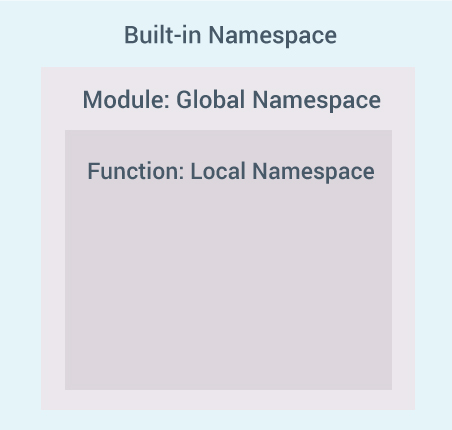
\includegraphics[width=0.65\textwidth]{figs/-namespaces-python.jpg}
%\end{figure}
%\end{frame}
%
%\begin{frame}[fragile]{An example of name space - dir() shows us the active names or attributes}
%\begin{minted}
%{python}
%a = 2.0
%
%def outter_fun():
%    b = 3.0
%    def inner_fun():
%        c = 3.0
%        print('inner function', dir())
%    inner_fun()
%    print('outter function', dir())
%
%outter_fun()
%print('script space', dir())
%\end{minted}
%\end{frame}
%
%\begin{frame}[fragile]{Functions and namespace}
%\begin{minted}
%{python}
%x = 2.0
%def print_x_new():
%    x = 1.0
%    print(x)
%print_x_new()
%\end{minted}
%Does this code change x?
%\end{frame}
%
%\begin{frame}[fragile]{Functions and namespace - global}
%\begin{minted}
%{python}
%x = 2.0
%def print_x_new():
%    global x
%    x = 1.0
%    print(x)
%print_x_new()
%\end{minted}
%Does this code change x?
%
%You need to declare \textit{global} before variable assignment
%
%\end{frame}
%
%\begin{frame}{Namespaces in Python is a good idea}
%\url{http://pclib.github.io/safari/program/learning-python/Text/ch29s04.html}
%
%Some good reading with Namespaces and Python.
%
%There is much to discuss but little time. 
%
%I recommended taking a look at the source code of how a library you use is organized. Such as numpy \url{https://github.com/numpy/numpy/tree/master/numpy}
%\end{frame}
%
%\begin{frame}{Python standard libraries}
%\url{https://docs.python.org/3/library/index.html}
%The Python libraries available with any Python installation.
%\begin{itemize}
%\item math - Mathematical function
%\item cmath - Mathematical functions for complex numbers
%\item itertools - functions for creating iterators for efficient looping
%\item pickle - Python object serialization (storing objects)
%\item csv - csv file read and write
%\item os - miscellaneous operating system interface
%\item and many more!
%\end{itemize}
%\end{frame}
%
%\begin{frame}{Special Python libraries we'll use in this course}
%\begin{itemize}
%\item numpy - fundamental package for scientific computing with Python
%\item matplotlib - Python 2D plotting library 
%\item scipy - Python-based ecosystem of open-source software for mathematics, science, and engineering
%\item sympy - symbolic math with Python
%\item sklearn - scikit-learn machine learning in Python
%\end{itemize}
%\end{frame}
%
%\begin{frame}[fragile]{Libraries and namespace - basic import}
%\begin{minted}
%{python}
%import math
%
%math.cos(math.pi)
%\end{minted}
%\begin{itemize}
%\item explicit import of the math library
%\item this is the most recommended type of import
%\item the functions of the math library exist in the math namespace
%\item run dir(math) to view all of the functions
%\item you access the functions using .
%\end{itemize}
%\end{frame}
%
%\begin{frame}[fragile]{Libraries and namespace - import as alias}
%\begin{minted}
%{python}
%import numpy as np
%
%np.cos(np.pi)
%\end{minted}
%\begin{itemize}
%\item sometimes it's inconvient to use the entire name of a library
%\item in this example we assign an alias np using as
%\item use the convention when importing libraries
%\item it is the convention to import numpy as np
%\end{itemize}
%\end{frame}
%
%\begin{frame}[fragile]{Libraries and namespace - explicit import of specific functions}
%\begin{minted}
%{python}
%from math import cos, pi
%
%cos(pi)
%\end{minted}
%\begin{itemize}
%\item sometimes it is useful to import just a few functions of a library
%\item in this case there will be no math namespace
%\item instead the functions cos and pi will occur in the local namespace
%\item from library import function1, function2, function3
%\end{itemize}
%\end{frame}
%
%\begin{frame}[fragile]{Libraries and namespace - implicit import of all functions}
%\begin{minted}
%{python}
%from sympy import *
%\end{minted}
%\begin{itemize}
%\item this imports all of the functions of sympy into the local namespace
%\item if this isn't officially recommended by your library, it could break default Python functions
%\item for instance from numpy import * would override max() and min() functions with the numpy max() and min() functions
%\end{itemize}
%\end{frame}
%
%\begin{frame}[fragile]{import os - useful for importing your operating system functions}
%\begin{minted}
%{python}
%import os
%os.getcwd()    # returns the current working directory as a string
%os.chdir(path) # changes the working directory to path
%os.listdir()   # returns a list of the entries in the current directory
%os.listdir(path)# a list of the entries in the path directory
%
%os.system()    # lets you run commands from your system terminal/prompt 
%'''
%os.system(command)
%    Execute the command in a subshell.
%    '''
%\end{minted}
%\end{frame}
%
%\begin{frame}[fragile]{The PyPA recommended tool for installing Python packages}
%pip is a tool for installing python packages -- execute pip from the anaconda prompt/terminal or the canopy prompt/terminal
%
%\url{https://pip.pypa.io/en/stable/quickstart/}
%
%Install a package:
%\begin{minted}
%{bash}
%$ pip install numpy 
%\end{minted}
%
%Upgrade a package:
%\begin{minted}
%{bash}
%$ pip install --upgrade numpy 
%\end{minted}
%
%Upgrade pip:
%\begin{minted}
%{bash}
%$ pip install --upgrade pip
%\end{minted}
%List what packages are outdated:
%\begin{minted}
%{bash}
%$ pip list --outdated
%\end{minted}
%\end{frame}
%
%\begin{frame}[fragile]{conda - if you installed Anaconda}
%conda is part of the Anaconda distribution and is a package, dependency manager for multiple languages \url{https://conda.io/docs/}
%
%You access conda from the Anaconda prompt/terminal
%
%To install a package:
%\begin{minted}
%{bash}
%$ conda install <package-name>
%\end{minted}
%
%To list the packages you have installed:
%\begin{minted}
%{bash}
%$ conda list
%\end{minted}
%
%To update all packages:
%\begin{minted}
%{bash}
%$ conda update --all
%\end{minted}
%
%To list all packages that are available
%\begin{minted}
%{bash}
%$ conda search
%\end{minted}
%\end{frame}
%
%\begin{frame}[fragile]{HW 03 - turn in one week from today in Canvas}
%Turn in the 5 questions as a single .py file onto canvas. Use comments to clearly indicate which question you are working on. Your filename should end as \_py2.py if you use Python2 and \_py3.py if you use Python3.
%\begin{enumerate}
%%\setcounter{enumi}{5}
%\item Open an Anaconda/Canopy prompt/terminal. Enter the command \textit{pip install pydoe} or (\textit{conda install pydoe} if you've installed anaconda) to install the pydoe package. This is a Python Design of Experiments library. In your .py file import pyDOE.
%\item Use the os library to print the current Python working directory. It is very useful to run system commands using os.system(). Import os. Run a system command to use the system's \textit{ping} program. If you are using Windows run the command \textit{ping -n 2 ufl.edu} or if you are using Linux/OS  \textit{ping -c 2 ufl.edu}. Hint: your command should be a string in Python.
%\item Compare math.pi to numpy.pi. Are these two representations of $\pi$ equivalent? Print the boolean statement True if they are, otherwise print False.
%\end{enumerate}
%
%\end{frame}
%
%
%\begin{frame}[fragile]{HW 03 - turn in one week from today in Canvas}
%\begin{enumerate}
%\setcounter{enumi}{3}
%\item Create a class called sphere. The object sphere requires a radius and mass to initialize. The attributes of the sphere should include the radius ($r$), mass ($m$), volume ($v$), surface area ($A$), and density ($\rho$). Initiate a new sphere name red with $r=1.7$ and $m=0.25$. Print dir(red). Print the volume, surface area, and density of red.
%\end{enumerate}
%\end{frame}
%
%\begin{frame}[fragile]{HW 03 - turn in one week from today in Canvas}
%\begin{enumerate}
%\setcounter{enumi}{4}
%\item The Python 3 print function adds some incredibly useful functionality
%\begin{minted}
%{python}
%x = 1.0; y = 2.0;
%print(x,y,sep = ' & ')
%\end{minted}
%will print \textit{1.0 \& 2.0}
%
%
%Given x
%\begin{minted}
%{python}
%x =   [[ 0,  1,  2,  3],[ 4,  5,  6,  7],
%[ 8,  9, 10, 11],[12, 13, 14, 15]]
%\end{minted}
%Use a for loop to iterate through the four lists in x. Each item in the list should be printed and separated by an \&. The following should be the output of your print. 
%
%
%0 \& 1 \& 2 \& 3
%
%4 \& 5 \& 6 \& 7
%
%8 \& 9 \& 10 \& 11
%
%12 \& 13 \& 14 \& 15
%
%\end{enumerate}
%Hint: from \_\_future\_\_ should go at the top of your script if you are using Python 2. 
%\end{frame}





\end{document}
